\documentclass{beamer}
\usetheme{Montpellier}
\usepackage{verbatim}	
\usepackage{natbib}

\title{Zone Plate tilt simulation }

\author{Sajid Ali\inst{1}}
% - Give the names in the same order as the appear in the paper.
% - Use the \inst{?} command only if the authors have different
%   affiliation.

\institute[NU] % (optional, but mostly needed)
{
  \inst{1}%
  Applied Physics\\
  Northwestern Univ}
% - Use the \inst command only if there are several affiliations.
% - Keep it simple, no one is interested in your street address.

\date{8 Aug 2018}
% - Either use conference name or its abbreviation.
% - Not really informative to the audience, more for people (including
%   yourself) who are reading the slides online

%\subject{Theoretical Computer Science}
% This is only inserted into the PDF information catalog. Can be left
% out. 

% If you have a file called "university-logo-filename.xxx", where xxx
% is a graphic format that can be processed by latex or pdflatex,
% resp., then you can add a logo as follows:

% \pgfdeclareimage[height=0.5cm]{university-logo}{university-logo-filename}
% \logo{\pgfuseimage{university-logo}}

% Delete this, if you do not want the table of contents to pop up at
% the beginning of each subsection:
\AtBeginSubsection[]
{
  \begin{frame}<beamer>{Outline}
    \tableofcontents[currentsection,currentsubsection]
  \end{frame}
}

% Let's get started
\begin{document}


\begin{frame}
  \titlepage
\end{frame}

\begin{frame}{Outline}
  \tableofcontents
  % You might wish to add the option [pausesections]
\end{frame}

% Section and subsections will appear in the presentation overview
% and table of contents.
\section{Multislice}

\subsection{Multislice basics}

\begin{frame}{What is multislice}
  \begin{itemize}
  \item Method to calculate x-ray wave propagation through arbitrary discrete objects
  \footnote{\cite{Li2015}\cite{Li2017}}
  \item Involves breaking up the object into multiple "slices" and alternate propagation between the slice and refraction at the slice.
  \end{itemize}
	  \begin{center}
  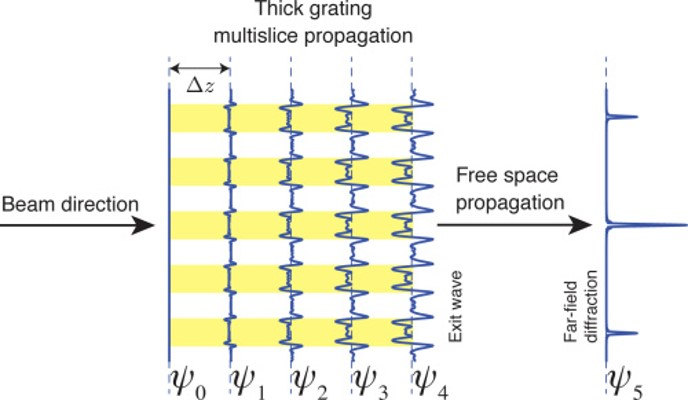
\includegraphics[scale=0.5]{multislice}
      	\end{center}
\end{frame}


\begin{frame}{Number of slices.}
\begin{itemize}
	\item Li et al\footnote{\cite{Li2017}} showed that by increasing the number of slices, the mulsitlice method gives identical results to CWT with the advantage that it can work with arbitrary structures on a discretized grid.
	\item It was empirically shown that the step size to achieve this is \\
	  \begin{center}
    $\Delta z = \frac{\epsilon_2}{{\epsilon_1}^2}\frac{{\Delta x}^2}{\lambda}$\\~\\
	 ($\Delta x$ is the pixel size, $\lambda$ is the wavelength and $\epsilon_1$, $\epsilon_2$ are $\approx$ 0.1.)
    	\end{center}
    \item Thus, we need more slices at lower energy. 

\end{itemize}
\end{frame}

\section{Zone plates}

\subsection{Introduction}
\begin{frame}{Need for multislice simulation}
\begin{itemize}
	\item Advances in nanofabrication processes have led to fabrication of zone plates with high aspect ratios\footnote{\cite{Chang2014},\cite{PhysRevLett.99.264801}}. As the thickness of zone plates increases and the outermost zone width decreases, aspect ratios as high as 500:1 have been achieved\footnote{\cite{Li2017b}}.
	\item These high aspect ratios have made the zone plates very sensitive to tilt alignment errors while also making them behave like volume gratings\footnote{\cite{Maser1992},\cite{Schneider1997}}.
	\item This makes previous results that calculate tilt tolerance that assume zone plates to be thin optical elements invalid and require new calculations for the same.
	
	
	
\end{itemize}
\end{frame}

\subsection{Tilt tolerance}
\begin{frame}{Previous results}
\begin{itemize}
	\item Myers\footnote{\cite{Myers1951}} and Young\footnote{\cite{Young1972}} had calculated the tilt tolerance using optical path lenghts. Jacobsen et al\footnote{\cite{Jacobsen1991}} took the depth of focus limits into account
	\item Jacobsen et al. \footnote{\cite{Chris_book}} approached the problem by relating the tilt angle to a factor of depth of focus. 
	\begin{center}
		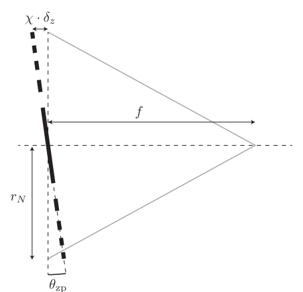
\includegraphics[scale=0.3]{chi_zp}
	\end{center}
	\item As stated earlier, these results don't take into account the thickness of the zone plates.
\end{itemize}
\end{frame}

\begin{frame}{Previous results}
	  \begin{center}
	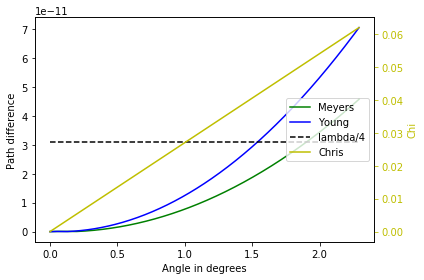
\includegraphics[scale=0.65]{lit_survey}
\end{center}
\end{frame}


\subsection{Implementation details}
\begin{frame}{Partial filling}
\begin{itemize}
	\item Pixel sizes are chosen to be no larger than 0.25 times the outermost zone width to ensure adequate sampling.
	\item Partial filling is done to avoid jagged edges. 
\end{itemize}
\begin{center}
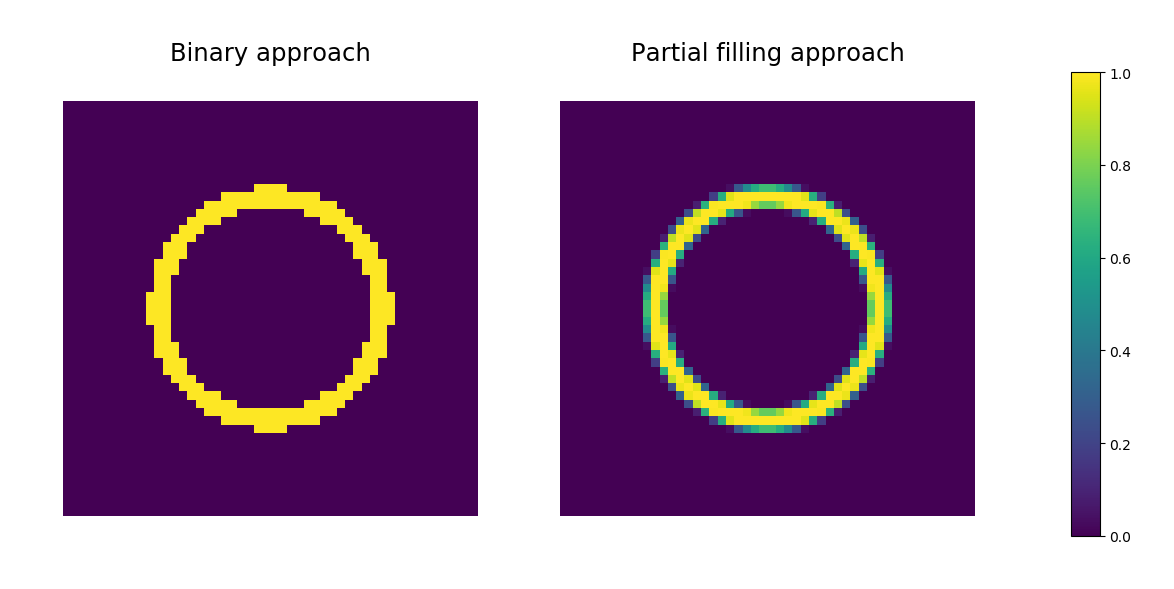
\includegraphics[scale=0.25]{partial_fill}
\end{center}
\end{frame}

\begin{frame}{Simulating tilt}
\begin{itemize}
\item To simulate tilt, the phase of the incoming plane wave is modified instead of
laboriously tilting the zone plate in three dimensions.
\item A plane wave input that is perfectly aligned with the zone plate would correspond to a grid where all the values are set to 1
\end{itemize}
\begin{center}
	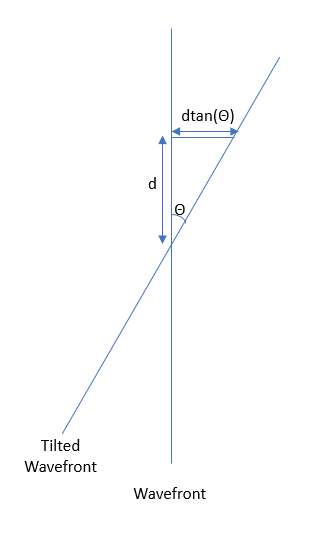
\includegraphics[scale=0.3]{tilt}
\end{center}
\end{frame}


\subsection{Results}

\begin{frame}{Dependance on number of zones}
\begin{itemize}
	\item Zone plate focal profiles along axis of tilt. Both zone plates are 8 microns thick but the one on the left has 200 zones and the one on the right has 500. 
\end{itemize}
\begin{center}
	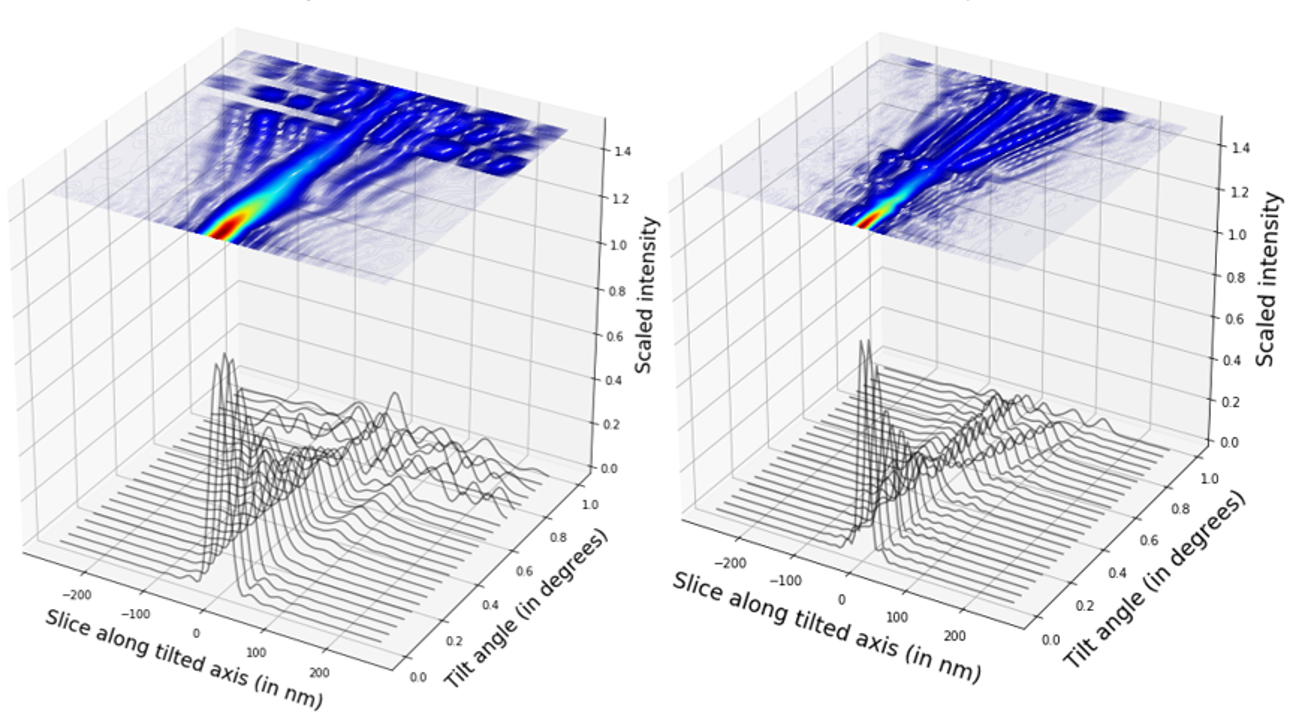
\includegraphics[scale=0.425]{8_200_500}
\end{center}
\end{frame}

\begin{frame}{Dependance on thickness}
\begin{itemize}
	\item Zone plate focal profiles along axis of tilt. Both have 200 zones while the one of the left is 0.5 microns thick and the one on the right is 10 microns thick.
	
\end{itemize}
\begin{center}
	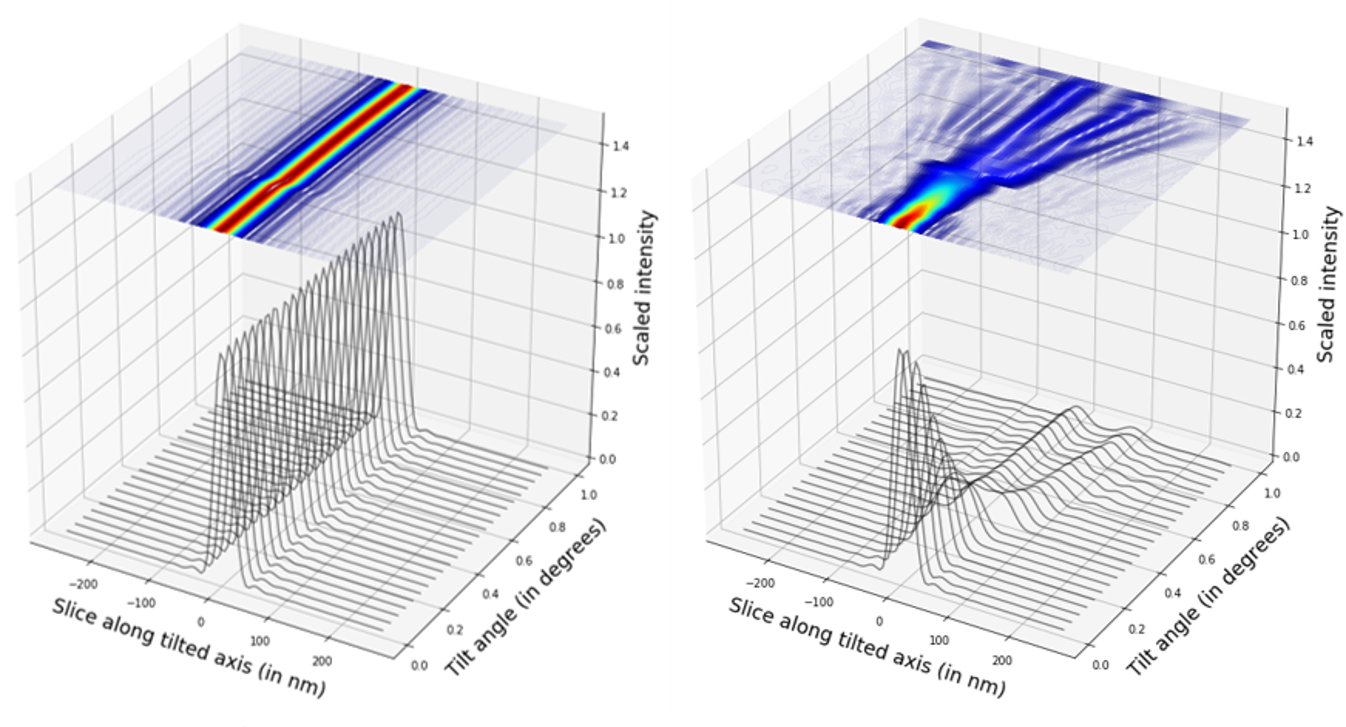
\includegraphics[scale=0.425]{200_half_ten}
\end{center}
\end{frame}


% Placing a * after \section means it will not show in the
% outline or table of contents.
\section*{Summary}

\begin{frame}{Summary}
  \begin{itemize}
  \item
  	Zone plate tilt tolerance depends on thickness of zone plate.
  \item
    Need better models to quantify tilt tolerance of zone plates.
  \item
    Multislice allows us to predict this.
  \end{itemize}  
  \begin{itemize}
  \item
    Future
    \begin{itemize}
    \item
	SRW integration ?
    \end{itemize}
  \end{itemize}
\end{frame}

\section*{Acknowledgements}

\begin{frame}{Acknowledgements}
\begin{itemize}
	\item
	\alert{Chris Jacobsen} XSD, APS.
	\item
	\alert{Kenan Li} SLAC National Accelerator Laboratory.
	\item
	\alert{Michael Wojcik} XSD, APS.
		
\end{itemize}
\end{frame}


% All of the following is optional and typically not needed. 
%\appendix
\renewcommand*{\bibfont}{\small}
\section{References}
\begin{frame}[t, allowframebreaks]
\frametitle{References}
\bibliographystyle{alpha}
\bibliography{zp_tilt}
\end{frame}

\end{document}

